% Options for packages loaded elsewhere
\PassOptionsToPackage{unicode}{hyperref}
\PassOptionsToPackage{hyphens}{url}
\PassOptionsToPackage{dvipsnames,svgnames,x11names}{xcolor}
%
\documentclass[
  letterpaper,
  DIV=11,
  numbers=noendperiod]{scrartcl}

\usepackage{amsmath,amssymb}
\usepackage{lmodern}
\usepackage{iftex}
\ifPDFTeX
  \usepackage[T1]{fontenc}
  \usepackage[utf8]{inputenc}
  \usepackage{textcomp} % provide euro and other symbols
\else % if luatex or xetex
  \usepackage{unicode-math}
  \defaultfontfeatures{Scale=MatchLowercase}
  \defaultfontfeatures[\rmfamily]{Ligatures=TeX,Scale=1}
\fi
% Use upquote if available, for straight quotes in verbatim environments
\IfFileExists{upquote.sty}{\usepackage{upquote}}{}
\IfFileExists{microtype.sty}{% use microtype if available
  \usepackage[]{microtype}
  \UseMicrotypeSet[protrusion]{basicmath} % disable protrusion for tt fonts
}{}
\makeatletter
\@ifundefined{KOMAClassName}{% if non-KOMA class
  \IfFileExists{parskip.sty}{%
    \usepackage{parskip}
  }{% else
    \setlength{\parindent}{0pt}
    \setlength{\parskip}{6pt plus 2pt minus 1pt}}
}{% if KOMA class
  \KOMAoptions{parskip=half}}
\makeatother
\usepackage{xcolor}
\setlength{\emergencystretch}{3em} % prevent overfull lines
\setcounter{secnumdepth}{-\maxdimen} % remove section numbering
% Make \paragraph and \subparagraph free-standing
\ifx\paragraph\undefined\else
  \let\oldparagraph\paragraph
  \renewcommand{\paragraph}[1]{\oldparagraph{#1}\mbox{}}
\fi
\ifx\subparagraph\undefined\else
  \let\oldsubparagraph\subparagraph
  \renewcommand{\subparagraph}[1]{\oldsubparagraph{#1}\mbox{}}
\fi

\usepackage{color}
\usepackage{fancyvrb}
\newcommand{\VerbBar}{|}
\newcommand{\VERB}{\Verb[commandchars=\\\{\}]}
\DefineVerbatimEnvironment{Highlighting}{Verbatim}{commandchars=\\\{\}}
% Add ',fontsize=\small' for more characters per line
\usepackage{framed}
\definecolor{shadecolor}{RGB}{241,243,245}
\newenvironment{Shaded}{\begin{snugshade}}{\end{snugshade}}
\newcommand{\AlertTok}[1]{\textcolor[rgb]{0.68,0.00,0.00}{#1}}
\newcommand{\AnnotationTok}[1]{\textcolor[rgb]{0.37,0.37,0.37}{#1}}
\newcommand{\AttributeTok}[1]{\textcolor[rgb]{0.40,0.45,0.13}{#1}}
\newcommand{\BaseNTok}[1]{\textcolor[rgb]{0.68,0.00,0.00}{#1}}
\newcommand{\BuiltInTok}[1]{\textcolor[rgb]{0.00,0.23,0.31}{#1}}
\newcommand{\CharTok}[1]{\textcolor[rgb]{0.13,0.47,0.30}{#1}}
\newcommand{\CommentTok}[1]{\textcolor[rgb]{0.37,0.37,0.37}{#1}}
\newcommand{\CommentVarTok}[1]{\textcolor[rgb]{0.37,0.37,0.37}{\textit{#1}}}
\newcommand{\ConstantTok}[1]{\textcolor[rgb]{0.56,0.35,0.01}{#1}}
\newcommand{\ControlFlowTok}[1]{\textcolor[rgb]{0.00,0.23,0.31}{#1}}
\newcommand{\DataTypeTok}[1]{\textcolor[rgb]{0.68,0.00,0.00}{#1}}
\newcommand{\DecValTok}[1]{\textcolor[rgb]{0.68,0.00,0.00}{#1}}
\newcommand{\DocumentationTok}[1]{\textcolor[rgb]{0.37,0.37,0.37}{\textit{#1}}}
\newcommand{\ErrorTok}[1]{\textcolor[rgb]{0.68,0.00,0.00}{#1}}
\newcommand{\ExtensionTok}[1]{\textcolor[rgb]{0.00,0.23,0.31}{#1}}
\newcommand{\FloatTok}[1]{\textcolor[rgb]{0.68,0.00,0.00}{#1}}
\newcommand{\FunctionTok}[1]{\textcolor[rgb]{0.28,0.35,0.67}{#1}}
\newcommand{\ImportTok}[1]{\textcolor[rgb]{0.00,0.46,0.62}{#1}}
\newcommand{\InformationTok}[1]{\textcolor[rgb]{0.37,0.37,0.37}{#1}}
\newcommand{\KeywordTok}[1]{\textcolor[rgb]{0.00,0.23,0.31}{#1}}
\newcommand{\NormalTok}[1]{\textcolor[rgb]{0.00,0.23,0.31}{#1}}
\newcommand{\OperatorTok}[1]{\textcolor[rgb]{0.37,0.37,0.37}{#1}}
\newcommand{\OtherTok}[1]{\textcolor[rgb]{0.00,0.23,0.31}{#1}}
\newcommand{\PreprocessorTok}[1]{\textcolor[rgb]{0.68,0.00,0.00}{#1}}
\newcommand{\RegionMarkerTok}[1]{\textcolor[rgb]{0.00,0.23,0.31}{#1}}
\newcommand{\SpecialCharTok}[1]{\textcolor[rgb]{0.37,0.37,0.37}{#1}}
\newcommand{\SpecialStringTok}[1]{\textcolor[rgb]{0.13,0.47,0.30}{#1}}
\newcommand{\StringTok}[1]{\textcolor[rgb]{0.13,0.47,0.30}{#1}}
\newcommand{\VariableTok}[1]{\textcolor[rgb]{0.07,0.07,0.07}{#1}}
\newcommand{\VerbatimStringTok}[1]{\textcolor[rgb]{0.13,0.47,0.30}{#1}}
\newcommand{\WarningTok}[1]{\textcolor[rgb]{0.37,0.37,0.37}{\textit{#1}}}

\providecommand{\tightlist}{%
  \setlength{\itemsep}{0pt}\setlength{\parskip}{0pt}}\usepackage{longtable,booktabs,array}
\usepackage{calc} % for calculating minipage widths
% Correct order of tables after \paragraph or \subparagraph
\usepackage{etoolbox}
\makeatletter
\patchcmd\longtable{\par}{\if@noskipsec\mbox{}\fi\par}{}{}
\makeatother
% Allow footnotes in longtable head/foot
\IfFileExists{footnotehyper.sty}{\usepackage{footnotehyper}}{\usepackage{footnote}}
\makesavenoteenv{longtable}
\usepackage{graphicx}
\makeatletter
\def\maxwidth{\ifdim\Gin@nat@width>\linewidth\linewidth\else\Gin@nat@width\fi}
\def\maxheight{\ifdim\Gin@nat@height>\textheight\textheight\else\Gin@nat@height\fi}
\makeatother
% Scale images if necessary, so that they will not overflow the page
% margins by default, and it is still possible to overwrite the defaults
% using explicit options in \includegraphics[width, height, ...]{}
\setkeys{Gin}{width=\maxwidth,height=\maxheight,keepaspectratio}
% Set default figure placement to htbp
\makeatletter
\def\fps@figure{htbp}
\makeatother

\KOMAoption{captions}{tableheading}
\makeatletter
\makeatother
\makeatletter
\makeatother
\makeatletter
\@ifpackageloaded{caption}{}{\usepackage{caption}}
\AtBeginDocument{%
\ifdefined\contentsname
  \renewcommand*\contentsname{Table of contents}
\else
  \newcommand\contentsname{Table of contents}
\fi
\ifdefined\listfigurename
  \renewcommand*\listfigurename{List of Figures}
\else
  \newcommand\listfigurename{List of Figures}
\fi
\ifdefined\listtablename
  \renewcommand*\listtablename{List of Tables}
\else
  \newcommand\listtablename{List of Tables}
\fi
\ifdefined\figurename
  \renewcommand*\figurename{Figure}
\else
  \newcommand\figurename{Figure}
\fi
\ifdefined\tablename
  \renewcommand*\tablename{Table}
\else
  \newcommand\tablename{Table}
\fi
}
\@ifpackageloaded{float}{}{\usepackage{float}}
\floatstyle{ruled}
\@ifundefined{c@chapter}{\newfloat{codelisting}{h}{lop}}{\newfloat{codelisting}{h}{lop}[chapter]}
\floatname{codelisting}{Listing}
\newcommand*\listoflistings{\listof{codelisting}{List of Listings}}
\makeatother
\makeatletter
\@ifpackageloaded{caption}{}{\usepackage{caption}}
\@ifpackageloaded{subcaption}{}{\usepackage{subcaption}}
\makeatother
\makeatletter
\@ifpackageloaded{tcolorbox}{}{\usepackage[many]{tcolorbox}}
\makeatother
\makeatletter
\@ifundefined{shadecolor}{\definecolor{shadecolor}{rgb}{.97, .97, .97}}
\makeatother
\makeatletter
\makeatother
\ifLuaTeX
  \usepackage{selnolig}  % disable illegal ligatures
\fi
\IfFileExists{bookmark.sty}{\usepackage{bookmark}}{\usepackage{hyperref}}
\IfFileExists{xurl.sty}{\usepackage{xurl}}{} % add URL line breaks if available
\urlstyle{same} % disable monospaced font for URLs
\hypersetup{
  pdftitle={HW2\_Qianru},
  colorlinks=true,
  linkcolor={blue},
  filecolor={Maroon},
  citecolor={Blue},
  urlcolor={Blue},
  pdfcreator={LaTeX via pandoc}}

\title{HW2\_Qianru}
\author{}
\date{}

\begin{document}
\maketitle
\ifdefined\Shaded\renewenvironment{Shaded}{\begin{tcolorbox}[borderline west={3pt}{0pt}{shadecolor}, breakable, enhanced, interior hidden, sharp corners, boxrule=0pt, frame hidden]}{\end{tcolorbox}}\fi

\hypertarget{hw2}{%
\subsection{HW2}\label{hw2}}

Replicate results of analysis from Lyubchich et al.~(2020) ``A
data-driven approach to detecting change points in linear regression
models'' in a Quatro document (newer version of Markdown).

\hypertarget{q1}{%
\subsection{Q1}\label{q1}}

Estimates in equations (8) and (9); retype the equations in this format
in your report

equations (8):

\[
\hat{y}_{1t}=-\underset{(0.405)}{\mathrm{0.980}}+\underset{(1.069·10^{-6})}{\mathrm{6.903·10^{−6}}}JanAprTNLoad_t,
\] equations (9):

\[
\hat{y}_{2t}=-\underset{(0.426)}{\mathrm{0.217}}+\underset{(1.360·10^{-6})}{\mathrm{5.596·10^{−6}}}JanMayTNLoad_t,
\]

\hypertarget{q2}{%
\subsection{Q2}\label{q2}}

Figure 3 (can provide a different look but preserve the superscripts in
axes labels and labels for the lines in A and D; format as subfigures
and not separate figures)

Early summer,respective residuals and sample autocorrelation functions
(ACFs) of the residuals

\begin{Shaded}
\begin{Highlighting}[]
\FunctionTok{library}\NormalTok{(ggplot2)}
\NormalTok{data}\OtherTok{=} \FunctionTok{read.csv}\NormalTok{(}\StringTok{\textquotesingle{}anoxia\_jmt3\_SL.csv\textquotesingle{}}\NormalTok{)}
\NormalTok{data}\SpecialCharTok{$}\NormalTok{fitted\_earlysummer}\OtherTok{=}\NormalTok{data}\SpecialCharTok{$}\NormalTok{JanAprTNLoad}\SpecialCharTok{*}\FloatTok{6.903}\SpecialCharTok{*}\NormalTok{(}\DecValTok{10}\SpecialCharTok{\^{}}\NormalTok{(}\SpecialCharTok{{-}}\DecValTok{6}\NormalTok{))}\SpecialCharTok{{-}}\FloatTok{0.980}
\NormalTok{data}\SpecialCharTok{$}\NormalTok{fitted\_latesummer}\OtherTok{=}\NormalTok{data}\SpecialCharTok{$}\NormalTok{JanMayTNLoad}\SpecialCharTok{*}\FloatTok{5.596}\SpecialCharTok{*}\NormalTok{(}\DecValTok{10}\SpecialCharTok{\^{}}\NormalTok{(}\SpecialCharTok{{-}}\DecValTok{6}\NormalTok{))}\SpecialCharTok{{-}}\FloatTok{0.217}

\NormalTok{data}\SpecialCharTok{$}\NormalTok{fitted\_earlysummer\_residuals}\OtherTok{=}\NormalTok{data}\SpecialCharTok{$}\NormalTok{EarlySummerAnoxicVol}\SpecialCharTok{{-}}\NormalTok{data}\SpecialCharTok{$}\NormalTok{fitted\_earlysummer}
\NormalTok{data}\SpecialCharTok{$}\NormalTok{fitted\_latesummer\_residuals}\OtherTok{=}\NormalTok{data}\SpecialCharTok{$}\NormalTok{LateSummerAnoxicVol}\SpecialCharTok{{-}}\NormalTok{data}\SpecialCharTok{$}\NormalTok{fitted\_latesummer}

\NormalTok{p1}\OtherTok{=}\FunctionTok{ggplot}\NormalTok{(data,}\FunctionTok{aes}\NormalTok{(}\AttributeTok{x=}\NormalTok{Year))}\SpecialCharTok{+}
  \FunctionTok{geom\_point}\NormalTok{(}\FunctionTok{aes}\NormalTok{(}\AttributeTok{y=}\NormalTok{EarlySummerAnoxicVol),}\AttributeTok{color=}\StringTok{"black"}\NormalTok{)}\SpecialCharTok{+}
  \FunctionTok{geom\_line}\NormalTok{(}\FunctionTok{aes}\NormalTok{(}\AttributeTok{y=}\NormalTok{EarlySummerAnoxicVol),}\AttributeTok{color=}\StringTok{"black"}\NormalTok{)}\SpecialCharTok{+}
  \FunctionTok{geom\_line}\NormalTok{(}\FunctionTok{aes}\NormalTok{(}\AttributeTok{y=}\NormalTok{fitted\_earlysummer),}\AttributeTok{color=}\StringTok{"blue"}\NormalTok{)}\SpecialCharTok{+}
  \FunctionTok{xlab}\NormalTok{(}\StringTok{"Year"}\NormalTok{) }\SpecialCharTok{+}
  \FunctionTok{ylab}\NormalTok{(}\FunctionTok{bquote}\NormalTok{(}\StringTok{\textquotesingle{}Early summer anoxic volume\textquotesingle{}}\NormalTok{ (km}\SpecialCharTok{\^{}}\DecValTok{3}\NormalTok{))) }\SpecialCharTok{+}
  \CommentTok{\#scale\_color\_manual(name = "Line",values = c(\textquotesingle{}black\textquotesingle{}, \textquotesingle{}blue\textquotesingle{}, \textquotesingle{}black\textquotesingle{}))+}
  \FunctionTok{theme\_classic}\NormalTok{()}\SpecialCharTok{+}
  \FunctionTok{annotate}\NormalTok{(}\AttributeTok{geom =} \StringTok{"text"}\NormalTok{, }\AttributeTok{x =} \DecValTok{1986}\NormalTok{, }\AttributeTok{y =} \FloatTok{2.2}\NormalTok{, }\AttributeTok{label =} \StringTok{"Fitted"}\NormalTok{,}\AttributeTok{color=}\StringTok{"blue"}\NormalTok{)}\SpecialCharTok{+}
  \FunctionTok{annotate}\NormalTok{(}\AttributeTok{geom =} \StringTok{"text"}\NormalTok{, }\AttributeTok{x =} \DecValTok{1986}\NormalTok{, }\AttributeTok{y =} \FloatTok{0.1}\NormalTok{, }\AttributeTok{label =} \StringTok{"Observed"}\NormalTok{,}\AttributeTok{color=}\StringTok{"black"}\NormalTok{)}
  
\NormalTok{p2}\OtherTok{=}\FunctionTok{ggplot}\NormalTok{(data,}\FunctionTok{aes}\NormalTok{(}\AttributeTok{x=}\NormalTok{Year))}\SpecialCharTok{+}
  \FunctionTok{geom\_point}\NormalTok{(}\FunctionTok{aes}\NormalTok{(}\AttributeTok{y=}\NormalTok{fitted\_earlysummer\_residuals),}\AttributeTok{color=}\StringTok{"black"}\NormalTok{)}\SpecialCharTok{+}
  \FunctionTok{geom\_line}\NormalTok{(}\FunctionTok{aes}\NormalTok{(}\AttributeTok{y=}\NormalTok{fitted\_earlysummer\_residuals),}\AttributeTok{color=}\StringTok{"black"}\NormalTok{)}\SpecialCharTok{+}
  \FunctionTok{xlab}\NormalTok{(}\StringTok{"Year"}\NormalTok{) }\SpecialCharTok{+}
  \FunctionTok{ylab}\NormalTok{(}\FunctionTok{bquote}\NormalTok{(}\StringTok{\textquotesingle{}Residuals\textquotesingle{}}\NormalTok{ (km}\SpecialCharTok{\^{}}\DecValTok{3}\NormalTok{))) }\SpecialCharTok{+}
  \FunctionTok{geom\_hline}\NormalTok{(}\AttributeTok{yintercept=}\DecValTok{0}\NormalTok{,}\AttributeTok{linetype=}\DecValTok{2}\NormalTok{)}\SpecialCharTok{+}
  \FunctionTok{theme\_classic}\NormalTok{()}

\NormalTok{p3}\OtherTok{=}\NormalTok{forecast}\SpecialCharTok{::}\FunctionTok{ggAcf}\NormalTok{(data}\SpecialCharTok{$}\NormalTok{fitted\_earlysummer\_residuals,}\DecValTok{15}\NormalTok{)}\SpecialCharTok{+}  
  \FunctionTok{ylim}\NormalTok{(}\SpecialCharTok{{-}}\FloatTok{0.4}\NormalTok{,}\FloatTok{0.4}\NormalTok{)}\SpecialCharTok{+}
  \FunctionTok{ylab}\NormalTok{(}\StringTok{"ACF of residuals"}\NormalTok{)}\SpecialCharTok{+}
  \FunctionTok{ggtitle}\NormalTok{(}\StringTok{\textquotesingle{}ACF\textquotesingle{}}\NormalTok{)}\SpecialCharTok{+}
  \FunctionTok{theme\_classic}\NormalTok{()}
\end{Highlighting}
\end{Shaded}

\begin{verbatim}
Registered S3 method overwritten by 'quantmod':
  method            from
  as.zoo.data.frame zoo 
\end{verbatim}

\begin{Shaded}
\begin{Highlighting}[]
\FunctionTok{library}\NormalTok{(ggplot2)}
\FunctionTok{library}\NormalTok{(cowplot)}
\FunctionTok{plot\_grid}\NormalTok{(p1, }\FunctionTok{plot\_grid}\NormalTok{(p2, p3), }\AttributeTok{ncol =} \DecValTok{1}\NormalTok{)}
\end{Highlighting}
\end{Shaded}

\begin{verbatim}
Warning: Removed 1 rows containing missing values (`geom_point()`).
\end{verbatim}

\begin{verbatim}
Warning: Removed 1 row containing missing values (`geom_line()`).
\end{verbatim}

\begin{verbatim}
Warning: Removed 1 rows containing missing values (`geom_point()`).
\end{verbatim}

\begin{verbatim}
Warning: Removed 1 row containing missing values (`geom_line()`).
\end{verbatim}

\begin{figure}[H]

{\centering 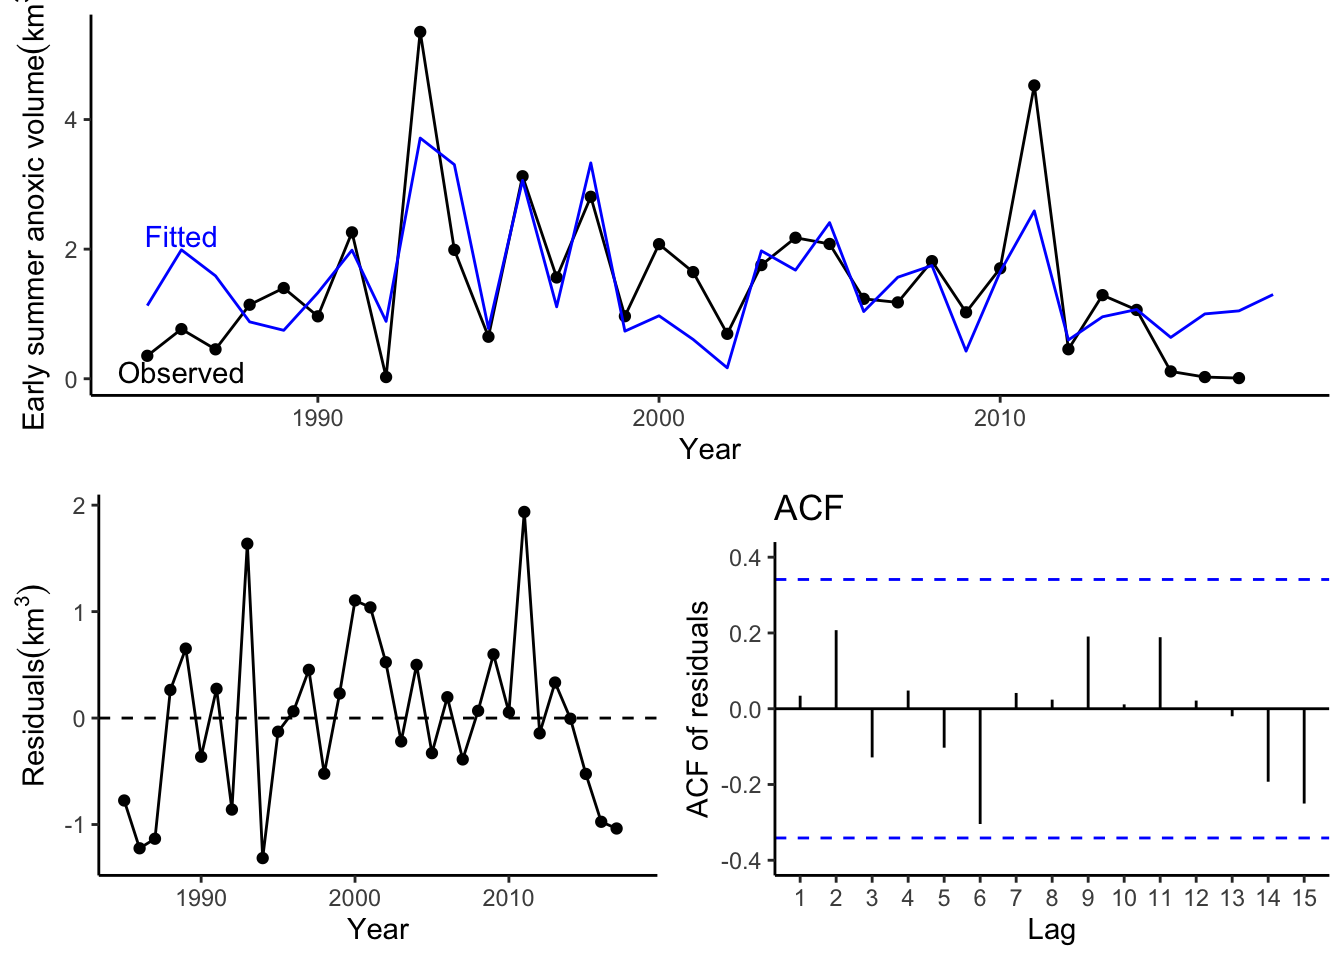
\includegraphics{HW2_files/figure-pdf/unnamed-chunk-1-1.pdf}

}

\end{figure}

Late summer,respective residuals and sample autocorrelation functions
(ACFs) of the residuals

\begin{Shaded}
\begin{Highlighting}[]
\NormalTok{p4}\OtherTok{=}\FunctionTok{ggplot}\NormalTok{(data,}\FunctionTok{aes}\NormalTok{(}\AttributeTok{x=}\NormalTok{Year))}\SpecialCharTok{+}
  \FunctionTok{geom\_point}\NormalTok{(}\FunctionTok{aes}\NormalTok{(}\AttributeTok{y=}\NormalTok{LateSummerAnoxicVol),}\AttributeTok{color=}\StringTok{"black"}\NormalTok{)}\SpecialCharTok{+}
  \FunctionTok{geom\_line}\NormalTok{(}\FunctionTok{aes}\NormalTok{(}\AttributeTok{y=}\NormalTok{LateSummerAnoxicVol),}\AttributeTok{color=}\StringTok{"black"}\NormalTok{)}\SpecialCharTok{+}
  \FunctionTok{geom\_line}\NormalTok{(}\FunctionTok{aes}\NormalTok{(}\AttributeTok{y=}\NormalTok{fitted\_latesummer),}\AttributeTok{color=}\StringTok{"blue"}\NormalTok{)}\SpecialCharTok{+}
  \FunctionTok{xlab}\NormalTok{(}\StringTok{"Year"}\NormalTok{) }\SpecialCharTok{+}
  \FunctionTok{ylab}\NormalTok{(}\FunctionTok{bquote}\NormalTok{(}\StringTok{\textquotesingle{}Late summer anoxic volume\textquotesingle{}}\NormalTok{ (km}\SpecialCharTok{\^{}}\DecValTok{3}\NormalTok{))) }\SpecialCharTok{+}
  \CommentTok{\#scale\_color\_manual(name = "Line",values = c(\textquotesingle{}black\textquotesingle{}, \textquotesingle{}blue\textquotesingle{}, \textquotesingle{}black\textquotesingle{}))+}
  \FunctionTok{theme\_classic}\NormalTok{()}\SpecialCharTok{+}
  \FunctionTok{annotate}\NormalTok{(}\AttributeTok{geom =} \StringTok{"text"}\NormalTok{, }\AttributeTok{x =} \DecValTok{1988}\NormalTok{, }\AttributeTok{y =} \FloatTok{1.1}\NormalTok{, }\AttributeTok{label =} \StringTok{"Fitted"}\NormalTok{,}\AttributeTok{color=}\StringTok{"blue"}\NormalTok{)}\SpecialCharTok{+}
  \FunctionTok{annotate}\NormalTok{(}\AttributeTok{geom =} \StringTok{"text"}\NormalTok{, }\AttributeTok{x =} \DecValTok{1986}\NormalTok{, }\AttributeTok{y =} \DecValTok{3}\NormalTok{, }\AttributeTok{label =} \StringTok{"Observed"}\NormalTok{,}\AttributeTok{color=}\StringTok{"black"}\NormalTok{)}
  
\NormalTok{p5}\OtherTok{=}\FunctionTok{ggplot}\NormalTok{(data,}\FunctionTok{aes}\NormalTok{(}\AttributeTok{x=}\NormalTok{Year))}\SpecialCharTok{+}
  \FunctionTok{geom\_point}\NormalTok{(}\FunctionTok{aes}\NormalTok{(}\AttributeTok{y=}\NormalTok{fitted\_latesummer\_residuals),}\AttributeTok{color=}\StringTok{"black"}\NormalTok{)}\SpecialCharTok{+}
  \FunctionTok{geom\_line}\NormalTok{(}\FunctionTok{aes}\NormalTok{(}\AttributeTok{y=}\NormalTok{fitted\_latesummer\_residuals),}\AttributeTok{color=}\StringTok{"black"}\NormalTok{)}\SpecialCharTok{+}
  \FunctionTok{xlab}\NormalTok{(}\StringTok{"Year"}\NormalTok{) }\SpecialCharTok{+}
  \FunctionTok{ylab}\NormalTok{(}\FunctionTok{bquote}\NormalTok{(}\StringTok{\textquotesingle{}Residuals\textquotesingle{}}\NormalTok{ (km}\SpecialCharTok{\^{}}\DecValTok{3}\NormalTok{))) }\SpecialCharTok{+}
  \FunctionTok{geom\_hline}\NormalTok{(}\AttributeTok{yintercept=}\DecValTok{0}\NormalTok{,}\AttributeTok{linetype=}\DecValTok{2}\NormalTok{)}\SpecialCharTok{+}
  \FunctionTok{theme\_classic}\NormalTok{()}

\NormalTok{p6}\OtherTok{=}\NormalTok{forecast}\SpecialCharTok{::}\FunctionTok{ggAcf}\NormalTok{(data}\SpecialCharTok{$}\NormalTok{fitted\_latesummer\_residuals,}\DecValTok{15}\NormalTok{)}\SpecialCharTok{+}  
  \FunctionTok{ylim}\NormalTok{(}\SpecialCharTok{{-}}\FloatTok{0.4}\NormalTok{,}\FloatTok{0.4}\NormalTok{)}\SpecialCharTok{+}
  \FunctionTok{ylab}\NormalTok{(}\StringTok{"ACF of residuals"}\NormalTok{)}\SpecialCharTok{+}
  \FunctionTok{ggtitle}\NormalTok{(}\StringTok{\textquotesingle{}ACF\textquotesingle{}}\NormalTok{)}\SpecialCharTok{+}
  \FunctionTok{theme\_classic}\NormalTok{()}

\FunctionTok{library}\NormalTok{(ggplot2)}
\FunctionTok{library}\NormalTok{(cowplot)}
\FunctionTok{plot\_grid}\NormalTok{(p4, }\FunctionTok{plot\_grid}\NormalTok{(p5, p6), }\AttributeTok{ncol =} \DecValTok{1}\NormalTok{)}
\end{Highlighting}
\end{Shaded}

\begin{verbatim}
Warning: Removed 1 rows containing missing values (`geom_point()`).
\end{verbatim}

\begin{verbatim}
Warning: Removed 1 row containing missing values (`geom_line()`).
\end{verbatim}

\begin{verbatim}
Warning: Removed 1 rows containing missing values (`geom_point()`).
\end{verbatim}

\begin{verbatim}
Warning: Removed 1 row containing missing values (`geom_line()`).
\end{verbatim}

\begin{figure}[H]

{\centering 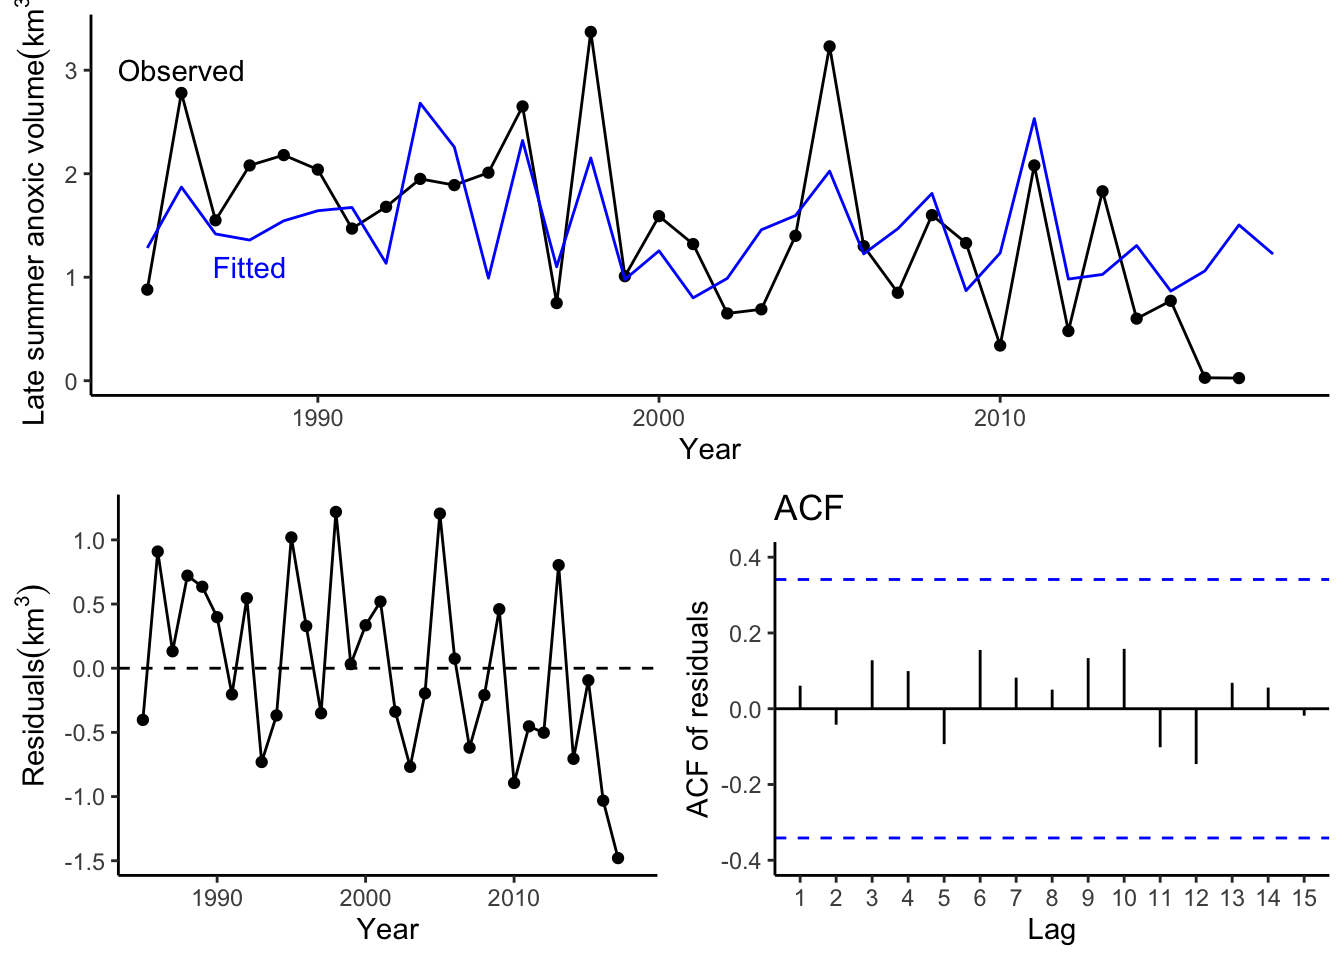
\includegraphics{HW2_files/figure-pdf/unnamed-chunk-2-1.pdf}

}

\end{figure}

\hypertarget{q3}{%
\subsection{Q3}\label{q3}}

Figure 4 (this figure can be presented as separate figures)
Classification and regression trees applied to residuals of (a) model
(8) for anoxic volumes in early summer, and (b) model (9) for anoxic
volumes in late summer. For each node, the average value of the
residuals is reported along with the node size expressed as percentage
of the total sample size T = 33

\begin{Shaded}
\begin{Highlighting}[]
\CommentTok{\#Classification and regression trees applied to residuals of model (8) for anoxic volumes in early summer}
\FunctionTok{library}\NormalTok{(rpart)}
\FunctionTok{library}\NormalTok{(rpart.plot)}
\FunctionTok{library}\NormalTok{(dplyr)}
\end{Highlighting}
\end{Shaded}

\begin{verbatim}

Attaching package: 'dplyr'
\end{verbatim}

\begin{verbatim}
The following objects are masked from 'package:stats':

    filter, lag
\end{verbatim}

\begin{verbatim}
The following objects are masked from 'package:base':

    intersect, setdiff, setequal, union
\end{verbatim}

\begin{Shaded}
\begin{Highlighting}[]
\CommentTok{\#classification}
\NormalTok{data\_early}\OtherTok{=}\FunctionTok{select}\NormalTok{(data,Year,fitted\_earlysummer\_residuals)}
\CommentTok{\# regression}
\NormalTok{m1 }\OtherTok{=} \FunctionTok{rpart}\NormalTok{(fitted\_earlysummer\_residuals }\SpecialCharTok{\textasciitilde{}}\NormalTok{ ., }
           \AttributeTok{control =} \FunctionTok{rpart.control}\NormalTok{(}\AttributeTok{maxdepth =} \DecValTok{2}\NormalTok{,}\AttributeTok{minbucket =} \DecValTok{4}\NormalTok{),}
           \AttributeTok{data =}\NormalTok{ data\_early)}
\FunctionTok{rpart.plot}\NormalTok{(m1)}
\end{Highlighting}
\end{Shaded}

\begin{figure}[H]

{\centering 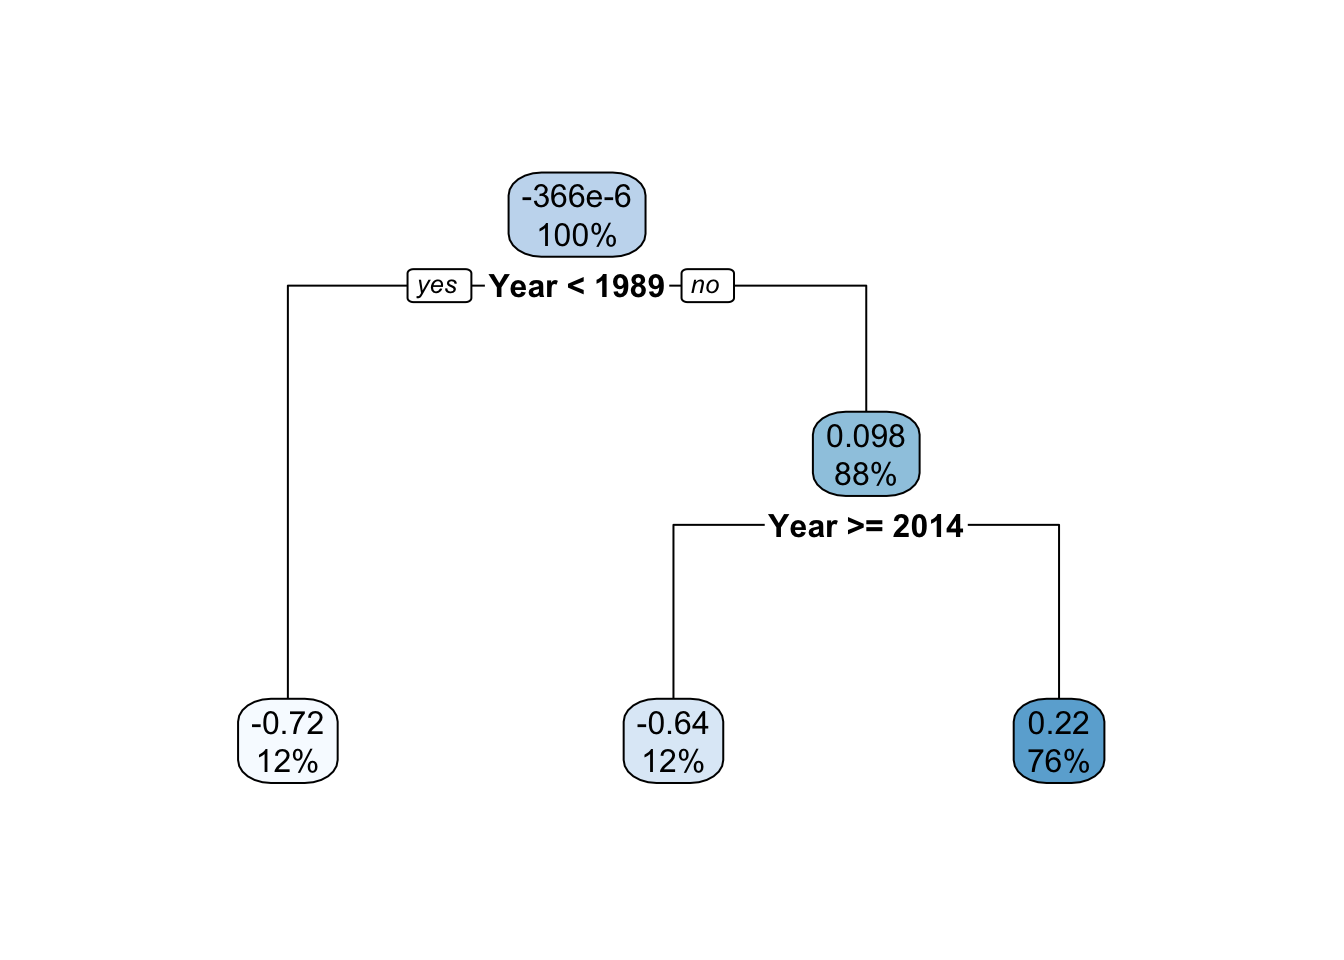
\includegraphics{HW2_files/figure-pdf/unnamed-chunk-3-1.pdf}

}

\end{figure}

\begin{Shaded}
\begin{Highlighting}[]
\CommentTok{\#Classification and regression trees applied to residuals of the model (9) for anoxic volumes in late summer}
\NormalTok{data\_late}\OtherTok{=}\FunctionTok{select}\NormalTok{(data,Year,fitted\_latesummer\_residuals)}
\CommentTok{\# regression}
\NormalTok{m2 }\OtherTok{=} \FunctionTok{rpart}\NormalTok{(fitted\_latesummer\_residuals }\SpecialCharTok{\textasciitilde{}}\NormalTok{ ., }
           \AttributeTok{control =} \FunctionTok{rpart.control}\NormalTok{(}\AttributeTok{maxdepth =} \DecValTok{2}\NormalTok{,}\AttributeTok{minbucket =} \DecValTok{4}\NormalTok{),}
           \AttributeTok{data =}\NormalTok{ data\_late)}
\FunctionTok{rpart.plot}\NormalTok{(m2)}
\end{Highlighting}
\end{Shaded}

\begin{figure}[H]

{\centering 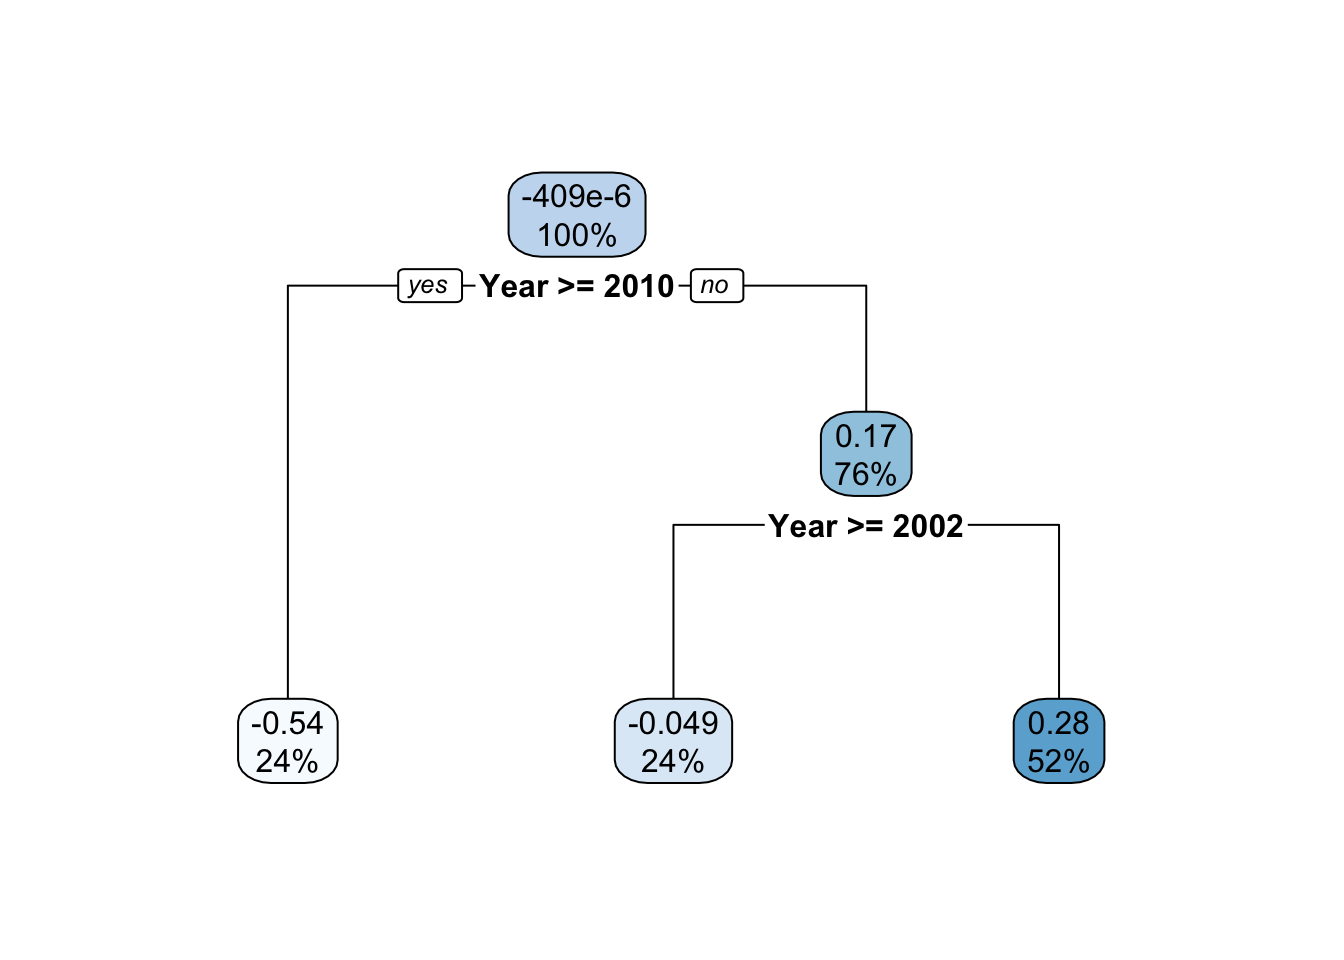
\includegraphics{HW2_files/figure-pdf/unnamed-chunk-4-1.pdf}

}

\end{figure}

\#\#Q4 Bootstrapped p-values (closely) corresponding to the two lines
for CART in Table 2

\begin{Shaded}
\begin{Highlighting}[]
\CommentTok{\#according to the method part in that paper, I will use mcusum\_test to calculate p value}
\CommentTok{\#1988{-}1985+1=4}
\CommentTok{\#2013{-}1985+1=29}
\FunctionTok{library}\NormalTok{(funtimes)}
\CommentTok{\#remove NA value}
\NormalTok{fitted\_earlysummer\_residuals\_new}\OtherTok{=}\FunctionTok{head}\NormalTok{(data}\SpecialCharTok{$}\NormalTok{fitted\_earlysummer\_residuals, }\SpecialCharTok{{-}}\DecValTok{1}\NormalTok{)}
\FunctionTok{mcusum\_test}\NormalTok{(}\AttributeTok{e=}\NormalTok{fitted\_earlysummer\_residuals\_new,}\AttributeTok{k=}\FunctionTok{c}\NormalTok{(}\DecValTok{4}\NormalTok{,}\DecValTok{29}\NormalTok{),}\AttributeTok{m=}\DecValTok{3}\NormalTok{,}\AttributeTok{B=}\DecValTok{10000}\NormalTok{,}\AttributeTok{ksm =} \ConstantTok{TRUE}\NormalTok{)}
\end{Highlighting}
\end{Shaded}

\begin{verbatim}

    Test for at-most-m changes in linear regression model

data:  fitted_earlysummer_residuals_new
M_T = 3.6447, mhat = 2, p-value = 0.0176
alternative hypothesis: at-most-2 changes exist
sample estimates:
$AR_order
[1] 0

$AR_coefficients
numeric(0)

$khat
[1]  4 29

$B
[1] 10000
\end{verbatim}

\begin{Shaded}
\begin{Highlighting}[]
\CommentTok{\#according to the method part in that paper, I will use mcusum\_test to calculate p value}
\CommentTok{\#2001{-}1985+1=17}
\CommentTok{\#2009{-}1985+1=25}
\FunctionTok{library}\NormalTok{(funtimes)}
\CommentTok{\#remove NA value}
\NormalTok{fitted\_latesummer\_residuals\_new}\OtherTok{=}\FunctionTok{head}\NormalTok{(data}\SpecialCharTok{$}\NormalTok{fitted\_latesummer\_residuals, }\SpecialCharTok{{-}}\DecValTok{1}\NormalTok{)}
\FunctionTok{mcusum\_test}\NormalTok{(}\AttributeTok{e=}\NormalTok{fitted\_latesummer\_residuals\_new,}\AttributeTok{k=}\FunctionTok{c}\NormalTok{(}\DecValTok{17}\NormalTok{,}\DecValTok{25}\NormalTok{),}\AttributeTok{m=}\DecValTok{3}\NormalTok{,}\AttributeTok{shortboot=}\ConstantTok{TRUE}\NormalTok{, }\AttributeTok{B=}\DecValTok{10000}\NormalTok{)}
\end{Highlighting}
\end{Shaded}

\begin{verbatim}

    Test for at-most-m changes in linear regression model

data:  fitted_latesummer_residuals_new
M_T = 2.7575, mhat = 2, p-value = 0.007899
alternative hypothesis: at-most-2 changes exist
sample estimates:
$AR_order
[1] 0

$AR_coefficients
numeric(0)

$khat
[1] 17 25

$B
[1] 10000
\end{verbatim}



\end{document}
